\documentclass[a4paper,12pt]{article}
\usepackage [utf8]{inputenc}
\usepackage [italian]{babel}
\usepackage{graphicx}
\usepackage{listings}
\usepackage{color}
\usepackage[hidelinks]{hyperref}
\usepackage{calc}
\usepackage{caption}
\usepackage{multicol}

\addtolength{\oddsidemargin}{-40pt}
\addtolength{\textwidth}{80pt}
\addtolength{\voffset}{-70pt}
\addtolength{\textheight}{120pt}


\graphicspath{ {../Schema concettuale} {../Schema logico relazionale} {../Piani di accesso} }
\lstset{inputpath=../Sorgenti SQL/}

\definecolor{codegreen}{rgb}{0,0.6,0}
\definecolor{codegray}{rgb}{0.5,0.5,0.5}
\definecolor{codepurple}{rgb}{0.58,0,0.82}
\definecolor{backcolour}{rgb}{0.95,0.95,0.92}

\lstdefinestyle{mystyle}{
    language=SQL,
    backgroundcolor=\color{backcolour},   
    commentstyle=\color{codegreen},
    keywordstyle=\color{magenta},
    numberstyle=\small\color{codegray},
    stringstyle=\color{codepurple},
    basicstyle=\ttfamily,
    breakatwhitespace=false,         
    breaklines=true,                 
    keepspaces=true,                 
    numbers=left,                    
    numbersep=10pt,                  
    showspaces=false,
    showstringspaces=false,
    showtabs=false,
    tabsize=4
}
\lstset{style=mystyle}

\addto\captionsitalian{%
\renewcommand{\lstlistingname}{Codice}}
\addto\captionsitalian{%
\renewcommand{\lstlistlistingname}{Elenco dei listati di codice}}


%%%%%%%%%%%%%%%%%%%%%%%  FRONTESPIZIO %%%%%%%%%%%%%%%%%%%%%%%

\title { \centering
\includegraphics[width=3cm]{ Stemma_unipi.png }\\{\small Università di Pisa\\Dipartimento di Informatica\\Corso di Laurea in Informatica\\[1cm]Corso di Basi di Dati (244AA), prof. Giorgio Ghelli\\[1.5cm]}Progetto ``Studio professionale fatture"\\Relazione finale\vspace{1cm} }

\author { \vspace{0.2cm}Candidati:\\Alessandro Antonelli\\\vspace{0.3cm}(matricola 507264, corso A)\\Tony Agosta\\(matricola 544090, corso A)}

\date { \vspace{1cm}Consegna: 25 marzo 2021\\Appello straordinario marzo 2021\\A.A. 2019/2020 }

\begin {document}
 \maketitle

 \clearpage
 
 \tableofcontents

\listoffigures

\lstlistoflistings

 \clearpage
 
%%%%%%%%%%%%%%%%%%%%%%%  CONTENUTO %%%%%%%%%%%%%%%%%%%%%%%

 \section{ Descrizione del dominio }

Uno studio professionale, inteso come studio di un commercialista, si occupa di gestire le pratiche in corso intestate ai suoi clienti, i quali presentano fatture di cui devono essere aiutati a pagare le tasse.

I clienti dello studio sono suddivisi in due sottoclassi partizione, Organizzazioni e Persone; le Organizzazioni possono essere titolari di 0, 1, o più pratiche, mentre tra le Persone, alcune sono titolari di 1 o più pratiche, altre non sono titolari di pratiche e ne seguono 1 o più per conto di una o più organizzazioni all’interno delle quali ricoprono un ruolo, tenendo conto che un ruolo può essere ricoperto da una o più persone, che un ruolo corrisponde a una e una sola organizzazione e che a una organizzazione corrispondono 1 o più ruoli.

Per ogni cliente che si rivolge allo studio viene aperta una pratica, a cui corrisponde un insieme di fatture. Questo vuol dire che una pratica, per esistere, deve essere intestata a un cliente ma un cliente può non avere pratiche in corso intestate in quel momento, in quanto alcuni clienti non sono titolari di pratiche ma possono seguirne una per conto di un’organizzazione per cui lavorano. Inoltre, ad ogni pratica possono essere associate più fatture e viceversa una fattura può essere relativa ad una sola pratica.

Una fattura può essere pagata con modalità di pagamenti differenti e a rate, questo vuol dire che un pagamento si può riferire ad una sola  fattura, ma una fattura può essere pagata, fino a raggiungere l’importo totale della fattura, da più pagamenti. A tal fine un cliente può effettuare più pagamenti, e un pagamento può essere effettuato da un solo cliente.

Ogni fattura è intestata a un solo cliente, e un cliente può avere 0, 1, o più fatture intestate. Un’organizzazione emette una o più fatture, e una fattura viene emessa sempre da una sola organizzazione.

Le classi individuate sono  7:
\begin{enumerate}
\item \textbf{Clienti}: rappresenta l’insieme di tutti i clienti dello studio professionale con le loro informazioni comuni.
\item \textbf{Persone}: rappresenta l’insieme delle persone sia come clienti dello studio professionale che, come persone, facenti parti di  una organizzazione. Specializza la classe “Clienti”.
\item \textbf{Organizzazioni}: rappresenta l’insieme delle organizzazioni clienti dello studio professionale. Specializza la classe “Clienti”.
\item \textbf{RuoliAziendali}:rappresenta l’insieme dei ruoli svolti da ogni persona che fa parte di una organizzazione.
\item \textbf{Pagamenti}: rappresenta l’insieme dei pagamenti con tutte le relative informazioni.
\item \textbf{Fatture}: rappresenta l’insieme delle fatture, con tutte le relative informazioni.
\item \textbf{Pratiche}: rappresenta l’insieme delle pratiche associate ai clienti.
\end{enumerate}

 \section{ Schema concettuale }

\begin{minipage}{\textwidth}
\begin{center}
\centering 
 \captionof{figure}{Schema concettuale a oggetti}
\centerline{
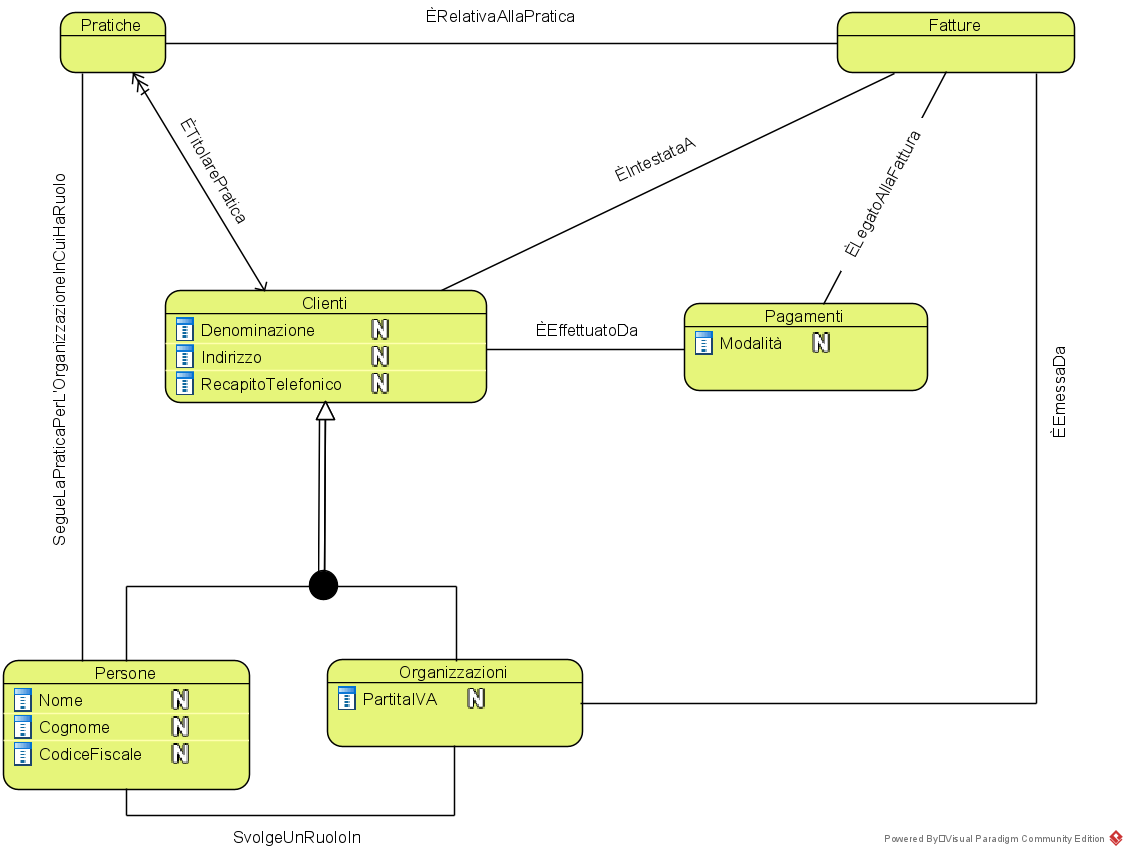
\includegraphics[width=\textwidth]{ Schema concettuale a oggetti.png }
}
\end{center}
\end{minipage}

 \subsection{ Vincoli }

\subsubsection{ Vincoli intrarelazionali }

\begin{itemize}
\item Tutti gli attributi (comprese le chiavi esterne) hanno il vincolo NOT NULL.

\item Il \textit{CodiceFiscale} di una \textit{Persona} deve essere lungo esattamente 16 caratteri.

\item L'\textit{Importo} di una \textit{Fattura} deve essere $> 0$.

\item La \textit{CifraPagata} di un \textit{Pagamento} deve essere $> 0$.

\item La \textit{PartitaIVA} di un'\textit{Organizzazione} deve essere di esattamente 11 caratteri.

\item Il \textit{RecapitoTelefonico} di un \textit{Cliente} non può essere lungo meno di 9 caratteri.
\end{itemize}

\subsubsection{ Vincoli interrelazionali }

\begin{itemize}
\item La \textit{CifraPagata} di un \textit{Pagamento} deve essere $\leq$ dell'\textit{Importo} della \textit{Fattura} a cui si riferisce.

\item Se il titolare di una \textit{Pratica} è un cliente che è una \textit{Organizzazione}, allora la \textit{Pratica} deve essere seguita da almeno un \textit{RuoloAziendale}.
\end{itemize}

 \section{ Schema logico relazionale }

 \subsection{ Formato grafico }

\begin{minipage}{\textwidth}
\textbf{Legenda}:

\includegraphics[width=0.5cm]{ Legenda chiave primaria.png } chiave primaria\hspace{1cm}

\includegraphics[width=0.5cm]{ Legenda chiave esterna.png } chiave esterna\hspace{1cm}

\includegraphics[width=0.5cm]{ Legenda attributo.png } attributo semplice

\begin{center}
\centering 
 \captionof{figure}{Schema logico relazionale}
\centerline{
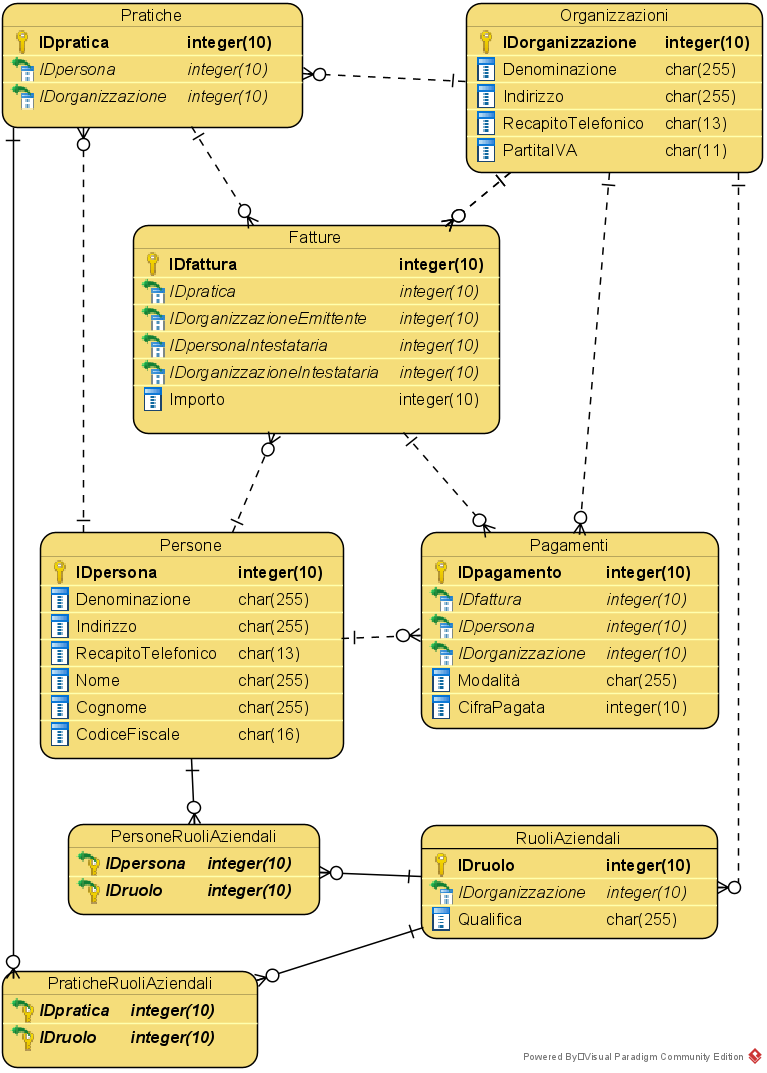
\includegraphics[width=\textwidth -4cm]{ Schema logico relazionale.png }
}
\end{center}
\end{minipage}

 \subsection{ Formato testuale }

\begin{itemize}
\item \textbf{Pratiche} (\underline{IDpratica}, IDpersona*, IDorganizzazione*)

\item \textbf{Fatture} (\underline{IDfattura}, IDpratica*, IDorganizzazioneEmittente*, IDpersonaIntestataria*, IDorganizzazioneIntestataria*, Importo, DataEmissione)

\item \textbf{Persone} (\underline{IDpersona}, Denominazione, Indirizzo, RecapitoTelefonico, Nome, Cognome, CodiceFiscale)

\item \textbf{Organizzazioni} (\underline{IDorganizzazione}, Denominazione, Indirizzo, RecapitoTelefonico, PartitaIVA)

\item \textbf{Pagamenti} (\underline{IDpagamento}, IDfattura*, IDpersona*, IDorganizzazione*, Modalità, CifraPagata, DataPagamento)

\item \textbf{RuoliAziendali} (\underline{IDruolo}, IDorganizzazione*, Qualifica)

\item \textbf{PersoneRuoliAziendali} (\underline{IDpersona*}, \underline{IDruolo*})

\item \textbf{PraticheRuoliAziendali} (\underline{IDpratica*}, \underline{IDruolo*})
\end{itemize}


 \subsection{ Dipendenze funzionali }

Tutte le relazioni rispettano la forma normale di Boyce-Codd (BCNF), di seguito si riportano le dipendenze funzionali di ciascuna:

\begin{itemize}
\item \textbf{Pratiche}\\È in BCNF perché IDpratica è chiave.
\begin{itemize}
\item IDpratica $\rightarrow$ IDpersona, IDorganizzazione
\end{itemize}

\item \textbf{Organizzazioni}\\È in BCNF perché IDorganizzazione è chiave, e PartitaIVA e RecapitoTelefonico, identificando una singola organizzazione, sono chiavi.
\begin{itemize}
\item IDorganizzazione $\rightarrow$ Denominazione, Indirizzo, RecapitoTelefonico, PartitaIVA
\item PartitaIVA $\rightarrow$ Denominazione, Indirizzo, RecapitoTelefonico, IDorganizzazione
\item RecapitoTelefonico $\rightarrow$ Denominazione, Indirizzo, PartitaIVA, IDorganizzazione
\end{itemize}

\item \textbf{Persone}\\È in BCNF perché IDpersona è chiave, e CodiceFiscale e RecapitoTelefonico, identificando una singola persona, sono chiavi.
\begin{itemize}
\item IDpersona $\rightarrow$ Denominazione, Indirizzo, RecapitoTelefonico, Nome, Cognome, CodiceFiscale
\item CodiceFiscale $\rightarrow$ Denominazione, Indirizzo, RecapitoTelefonico, Nome, Cognome, IDpersona
\item RecapitoTelefonico $\rightarrow$ Denominazione, Indirizzo, Nome, Cognome, CodiceFiscale, IDpersona
\end{itemize}

\item \textbf{PersoneRuoliAziendali} è in BCNF perché non ha dipendenze non banali.

\item \textbf{PraticheRuoliAziendali} è in BCNF perché non ha dipendenze non banali.

\item \textbf{RuoliAziendali}\\È in BCNF perché IDruolo è chiave.
\begin{itemize}
\item IDruolo $\rightarrow$ Qualifica, IDorganizzazione
\end{itemize}

\item \textbf{Fatture}\\È in BCNF perché IDfattura è chiave, e perché IDPratica identifica un unico cliente (persona o organizzazione), come verificabile nello schema concettuale.

\begin{itemize}
\item IDfattura $\rightarrow$ Importo, IDpratica, IDorganizzazioneEmittente, IDpersonaIntestataria, IDorganizzazioneIntestataria, DataEmissione

\item IDpratica $\rightarrow$ IDpersonaIntestataria, IDorganizzazioneIntestataria
\end{itemize}

\item \textbf{Pagamenti}\\È in BCNF perché IDpagamento è chiave.

\begin{itemize}
\item IDpagamento $\rightarrow$ Modalità, CifraPagata, IDfattura, IDpersona, IDorganizzazione, DataPagamento
\end{itemize}

\end{itemize}

 \section{ Interrogazioni }


 \subsection{ Uso di proiezione, join e restrizione }
Stampa le persone intestatarie di fatture i cui importi sono $> 100$:

\begin{minipage}{\textwidth}
\lstinputlisting[caption=Query 1,title=Codice query 1:]{1.sql}
\end{minipage}


 \subsection{ Uso di group by con having, where e sort }

Stampa il totale per ogni modalità di pagamento dato dai pagamenti in cui CifraPagata $> 10$ e $< 10000$, e ordinate in base al totale:

\begin{minipage}{\textwidth}
\lstinputlisting[caption=Query 2,title=Codice query 2:]{2.sql}
\end{minipage}


 \subsection{ Uso di join, group by con having e where }

Stampa il codice fiscale delle persone intestatarie di più di 3 fatture il cui importo è $> 1000$:

\begin{minipage}{\textwidth}
\lstinputlisting[caption=Query 3,title=Codice query 3:]{3.sql}
\end{minipage}

 \subsection{ Uso di select annidata con quantificazione esistenziale }

Stampa le organizzazioni che hanno emesso almeno una fattura con un importo $> 100$:

\begin{minipage}{\textwidth}
\lstinputlisting[caption=Query 4,title=Codice query 4:]{4.sql}
\end{minipage}

 \subsection{ Uso di select annidata con quantificazione universale }

Stampa le fatture che non sono state pagate in contanti:

\begin{minipage}{\textwidth}
\lstinputlisting[caption=Query 5,title=Codice query 5:]{5.sql}
\end{minipage}

 \subsection{ Uso di subquery di confronto quantificato usando una subquery }

Stampa i pagamenti effettuati tramite bonifico il cui importo è maggiore del pagamento massimo effettuato tramite assegno:

\begin{minipage}{\textwidth}
\lstinputlisting[caption=Query 6,title=Codice query 6:]{6.sql}
\end{minipage}

 \section{ Piani di accesso }

                    %%%%%%%%%%
 \subsection{ Piani di accesso logico }

 \subsubsection{ Query 1) }

\begin{minipage}{\textwidth}
\begin{multicols}{2}

\null \vfill
\lstinputlisting[basicstyle=\footnotesize,nolol,title=Codice query:]{1.sql}
\vfill \null

\columnbreak

 \captionof{figure}[Piano di accesso logico della query 1]{Piano di accesso logico:}
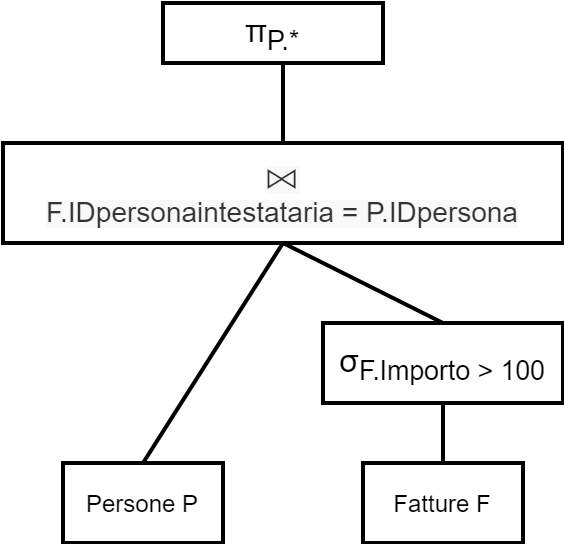
\includegraphics[height=7cm]{ Albero logico 1.png }

\end{multicols}
\end{minipage}

 \subsubsection{ Query 2) }

\begin{minipage}{\textwidth}
\begin{multicols}{2}

\null \vfill
\lstinputlisting[basicstyle=\footnotesize,nolol,title=Codice query:]{2.sql}
\vfill \null

\columnbreak

 \captionof{figure}[Piano di accesso logico della query 2]{Piano di accesso logico:}
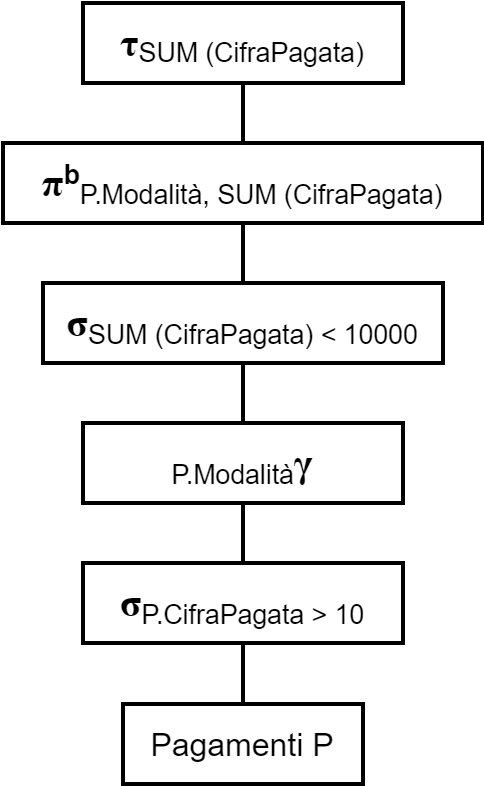
\includegraphics[height=10cm]{ Albero logico 2.png }
\end{multicols}
\end{minipage}

 \subsubsection{ Query 3) }

\begin{minipage}{\textwidth}
\begin{multicols}{2}

\null \vfill
\lstinputlisting[basicstyle=\footnotesize,nolol,title=Codice query:]{3.sql}
\vfill \null

\columnbreak

 \captionof{figure}[Piano di accesso logico della query 3]{Piano di accesso logico:}
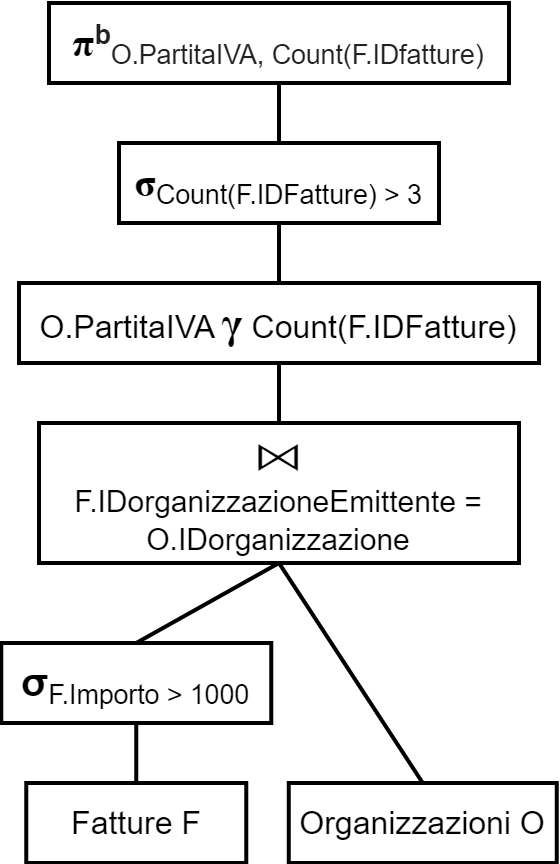
\includegraphics[height=10cm]{ Albero logico 3.png }
\end{multicols}
\end{minipage}

                    %%%%%%%%%%%%%%%%%%
 \subsection{ Piani di accesso fisico senza uso di indici }

 \subsubsection{ Query 1) }

\vspace{-0.3cm}\hspace{-0.7cm}
\begin{minipage}{\textwidth}
\begin{multicols}{2}

\null \vfill
Piano di accesso logico:

\vspace{0.3cm}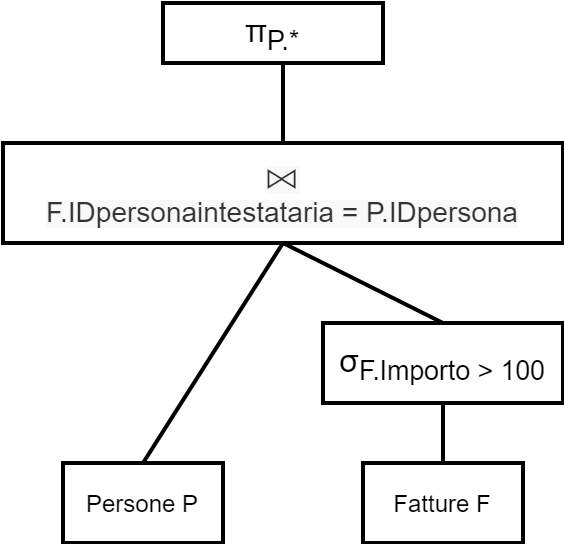
\includegraphics[height=7.5cm]{ Albero logico 1.png }
\vfill \null

\columnbreak

 \captionof{figure}[Piano di accesso fisico della query 1 senza indici]{Piano di accesso fisico senza indici:}
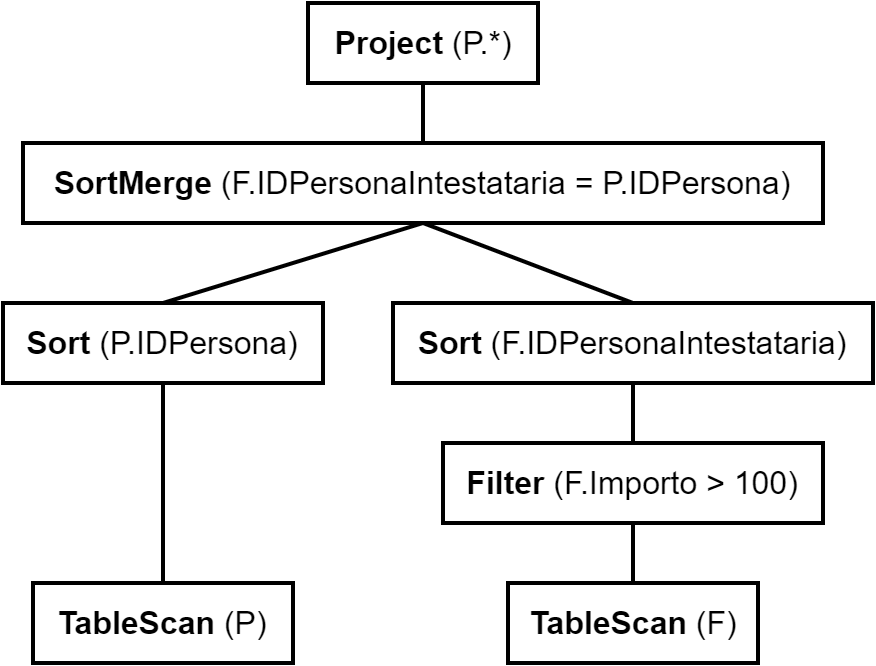
\includegraphics[height=7.5cm]{ Albero fisico 1.png }
\end{multicols}
\end{minipage}

 \subsubsection{ Query 2) }

\vspace{-0.3cm}\begin{minipage}{\textwidth}
\begin{multicols}{2}

\null \vfill
Piano di accesso logico:

\vspace{0.3cm}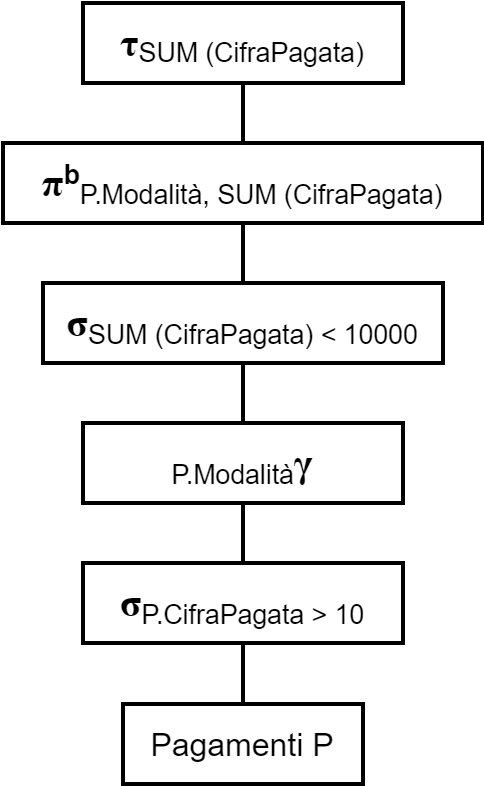
\includegraphics[height=9.5cm]{ Albero logico 2.png }
\vfill \null

\columnbreak

 \captionof{figure}[Piano di accesso fisico della query 2 senza indici]{Piano di accesso fisico senza indici:}
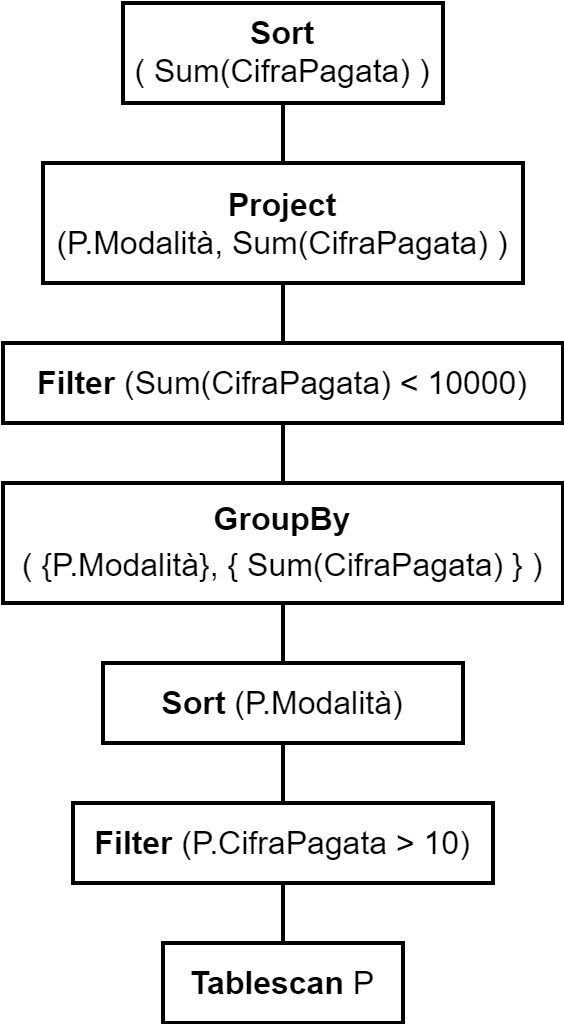
\includegraphics[height=10cm]{ Albero fisico 2.png }
\end{multicols}
\end{minipage}

 \subsubsection{ Query 3) }

\vspace{-0.3cm}\begin{minipage}{\textwidth}
\begin{multicols}{2}

\null \vfill
Piano di accesso logico:

\vspace{0.3cm}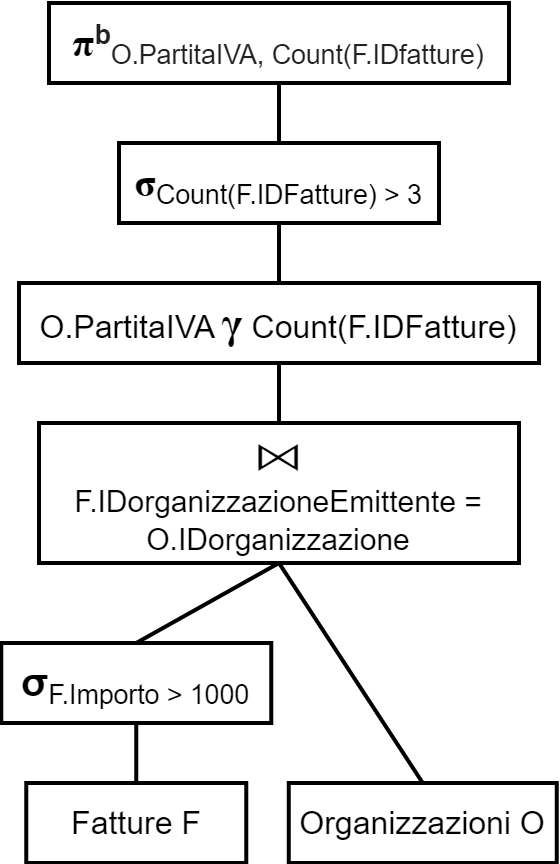
\includegraphics[height=10cm]{ Albero logico 3.png }
\vfill \null

\columnbreak

 \captionof{figure}[Piano di accesso fisico della query 3 senza indici]{Piano di accesso fisico senza indici:}
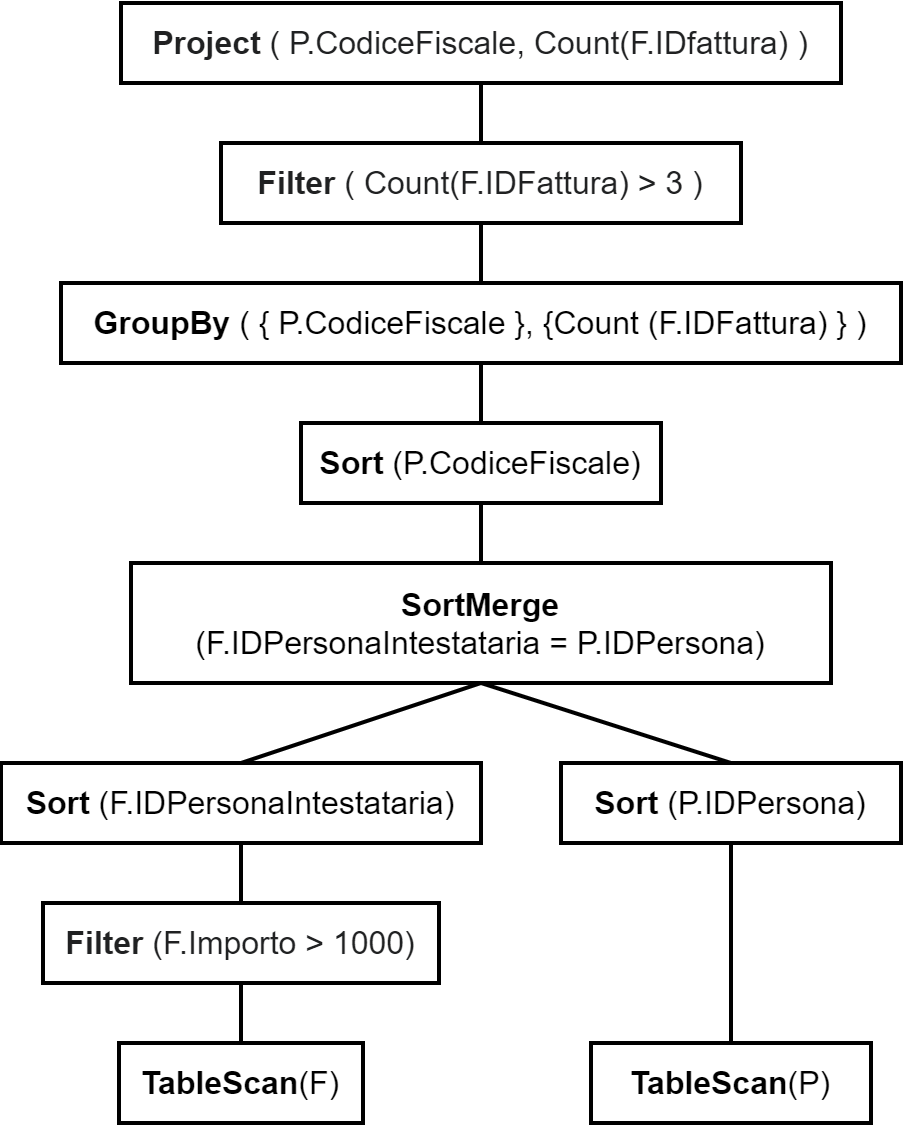
\includegraphics[height=10cm]{ Albero fisico 3.png }
\end{multicols}
\end{minipage}

                    %%%%%%%%%%%%%%%%%
 \subsection{ Piani di accesso fisico con uso di indici }

 \subsubsection{ Query 1) }

\vspace{-0.3cm}\hspace{-0.7cm}
\begin{minipage}{\textwidth}
\begin{multicols}{2}

\null \vfill
Piano di accesso fisico senza indici:

\vspace{0.3cm}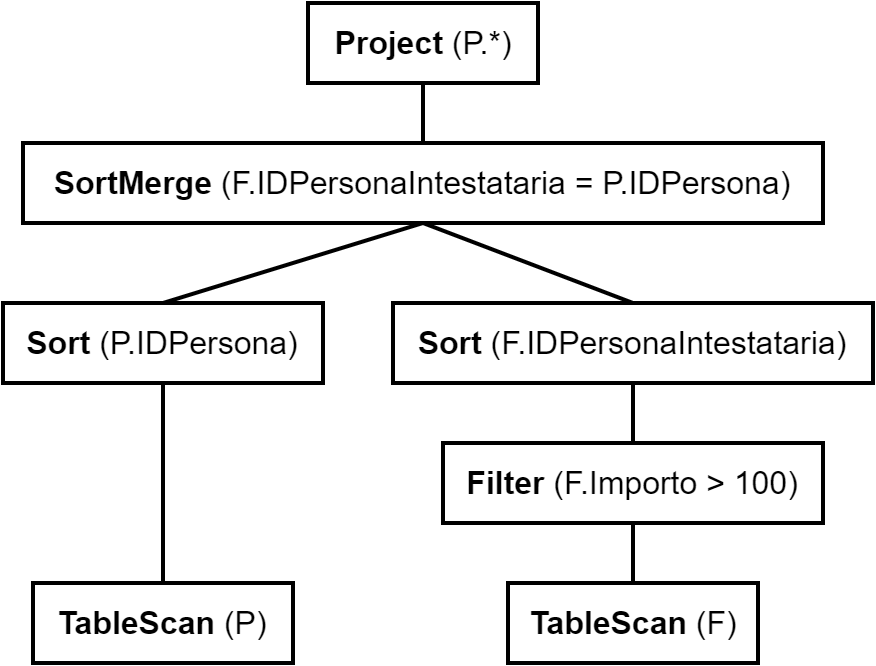
\includegraphics[height=5.7cm]{ Albero fisico 1.png }
\vfill \null

\columnbreak

 \captionof{figure}[Piano di accesso fisico della query 1 con indici]{Piano di accesso fisico con indici:}
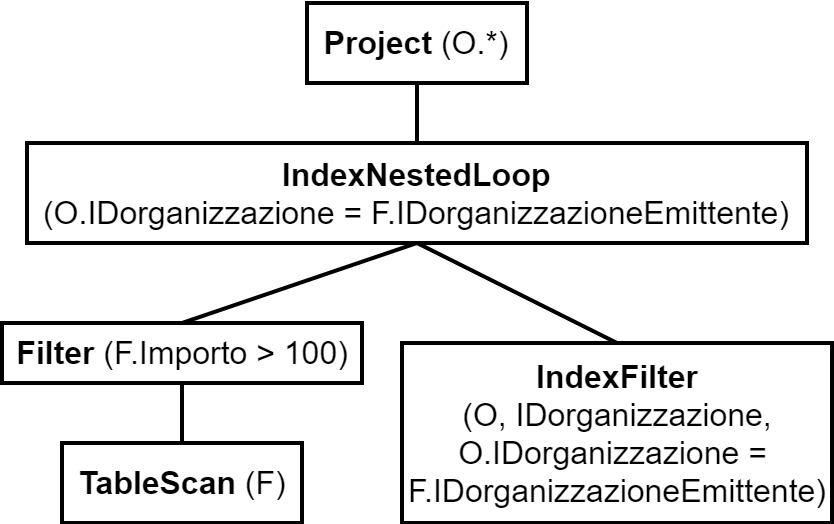
\includegraphics[height=5.7cm]{ Albero fisico indici 1.png }

Si suppone di disporre di un indice sull'attributo IDPersona.

\end{multicols}
\end{minipage}

 \subsubsection{ Query 2) }

\vspace{-0.3cm}\begin{minipage}{\textwidth}
\begin{multicols}{2}

\null \vfill
Piano di accesso fisico senza indici:

\vspace{0.3cm}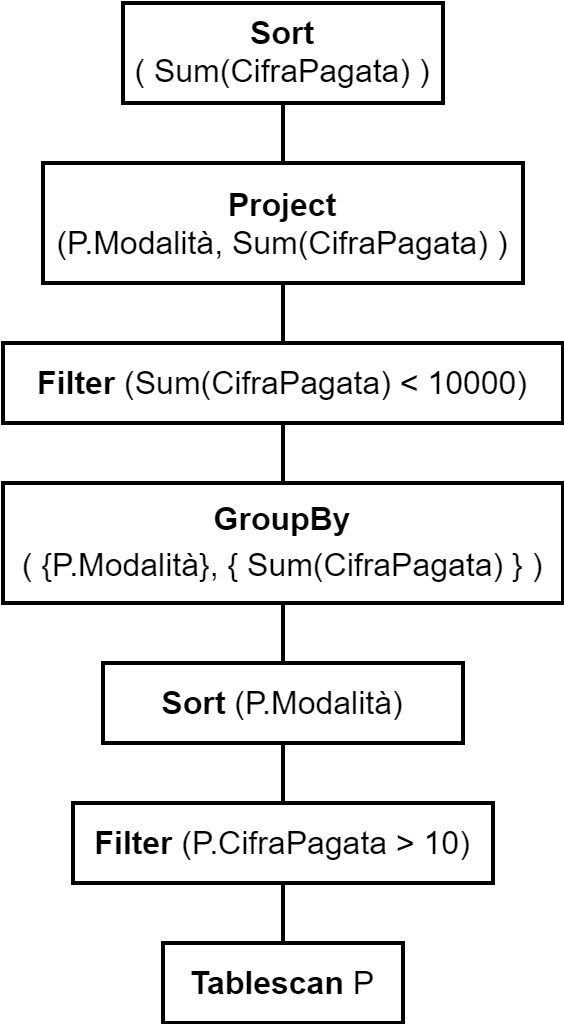
\includegraphics[height=10cm]{ Albero fisico 2.png }
\vfill \null

\columnbreak

 \captionof{figure}[Piano di accesso fisico della query 2 con indici]{Piano di accesso fisico con indici:}
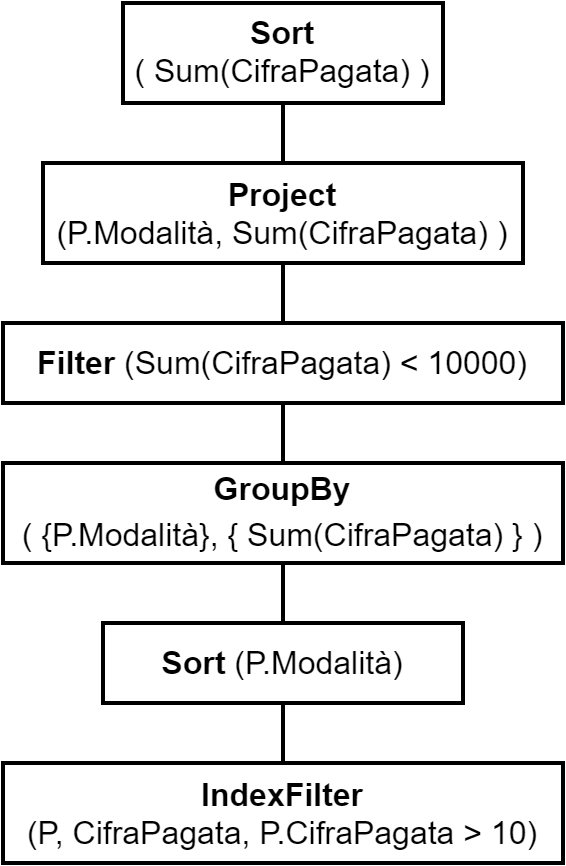
\includegraphics[height=10.5cm]{ Albero fisico indici 2.png }

Si suppone di disporre di un indice sull'attributo CifraPagata.

\end{multicols}
\end{minipage}

 \subsubsection{ Query 3) }

\vspace{-0.3cm}\hspace{-1cm}
\begin{minipage}{\textwidth}
\begin{multicols}{2}

\null \vfill
Piano di accesso fisico senza indici:

\vspace{0.3cm}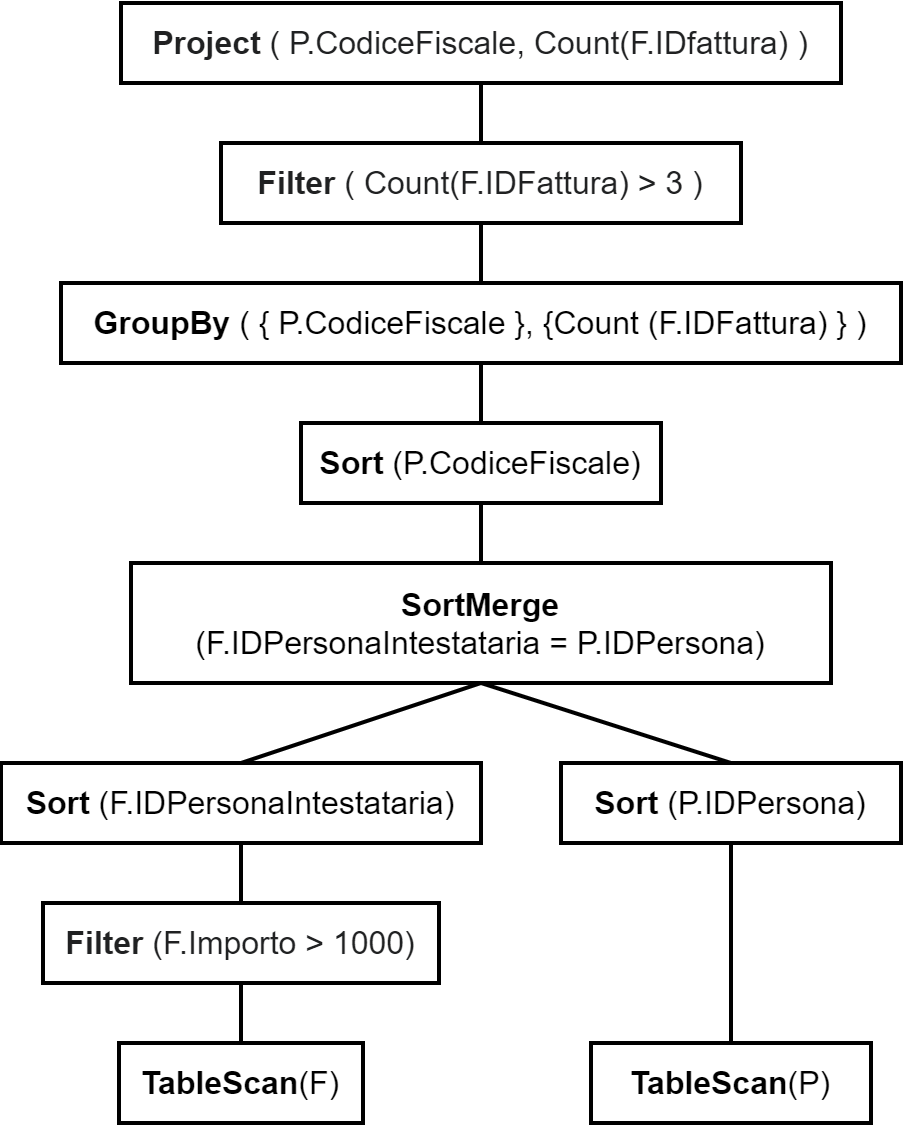
\includegraphics[height=9.5cm]{ Albero fisico 3.png }
\vfill \null

\columnbreak

 \captionof{figure}[Piano di accesso fisico della query 3 con indici]{Piano di accesso fisico con indici:}
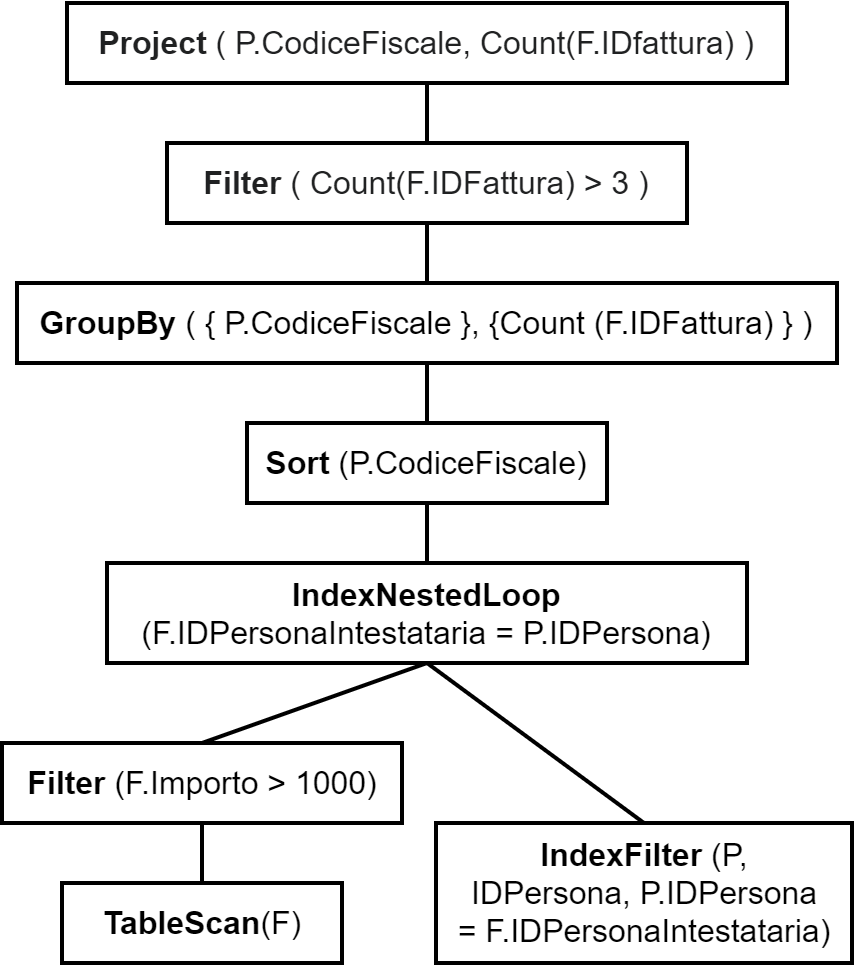
\includegraphics[height=11cm]{ Albero fisico indici 3.png }

Si suppone di disporre di un indice sull'attributo IDPersona.

\end{multicols}
\end{minipage}

\end{document}